    Tenemos que demostrar que el vector excentricidad lleva el sentido hacia la periapsis.


    \begin{minipage}{.45\textwidth} 	
        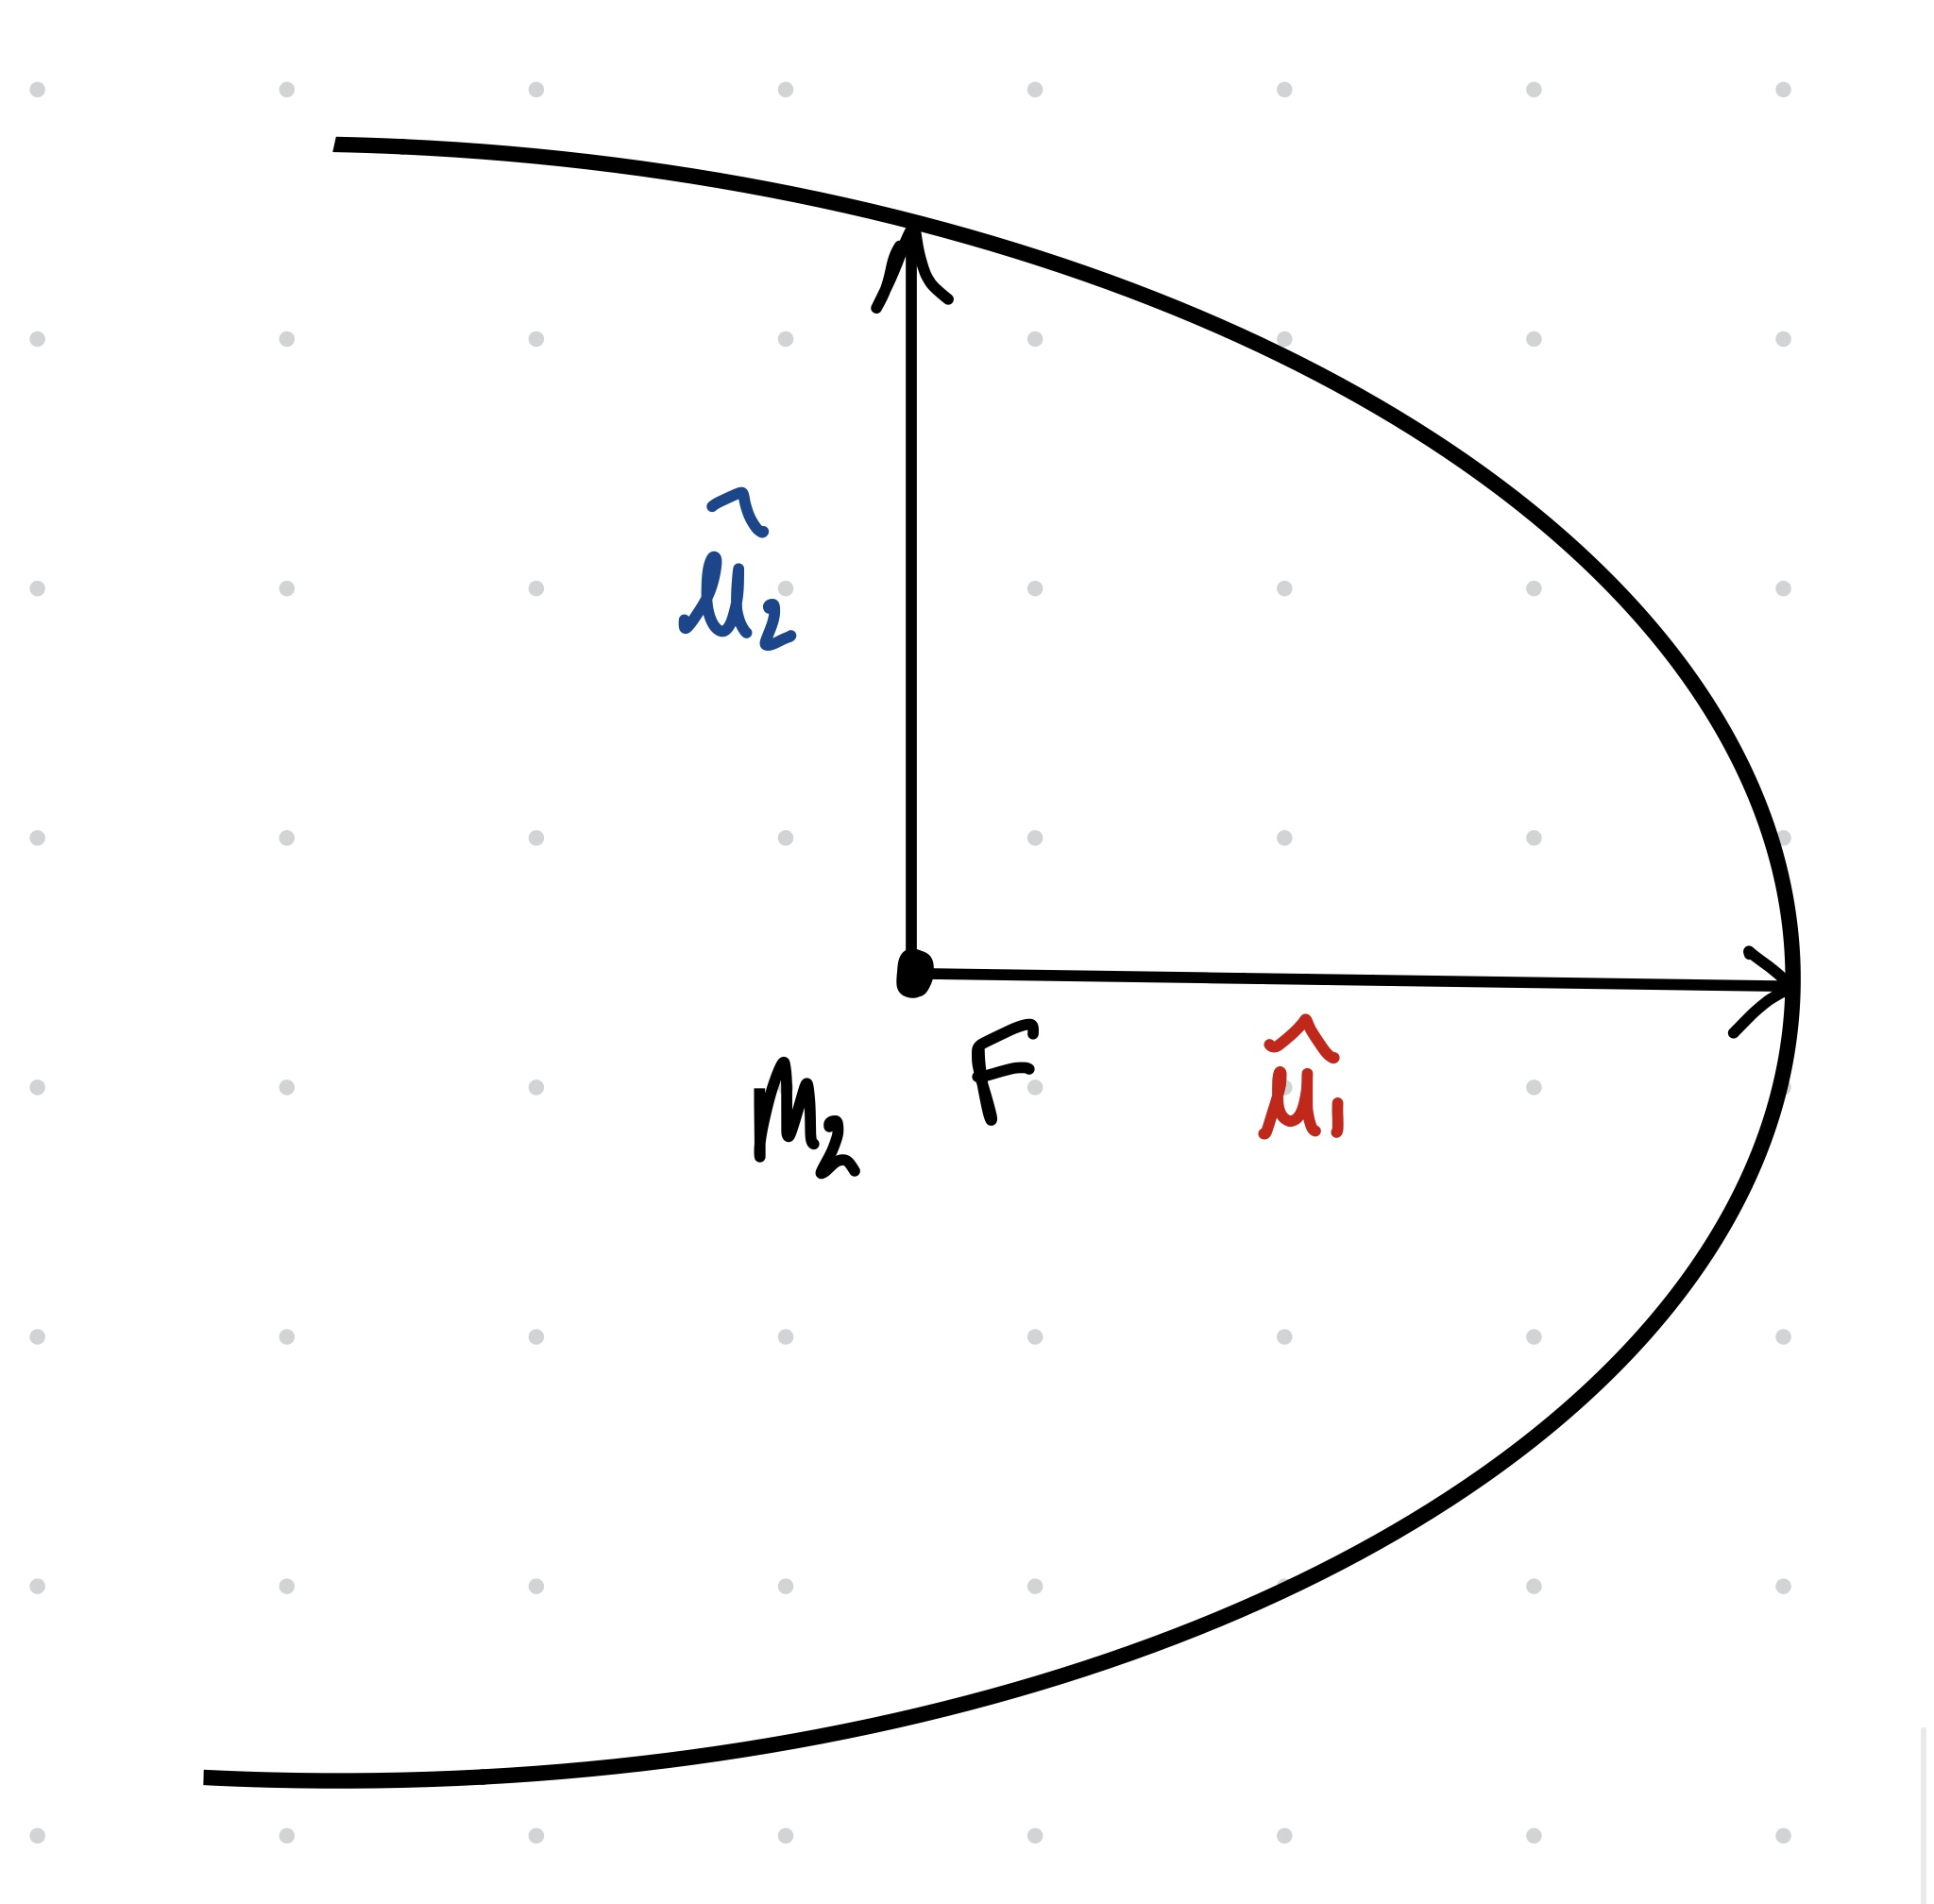
\includegraphics[width=0.8\textwidth]{Cuerpo/Imagenes/02_Ejercicio_1_1.jpg}
    \end{minipage}	\hfill
    \begin{minipage}{0.45\textwidth}
        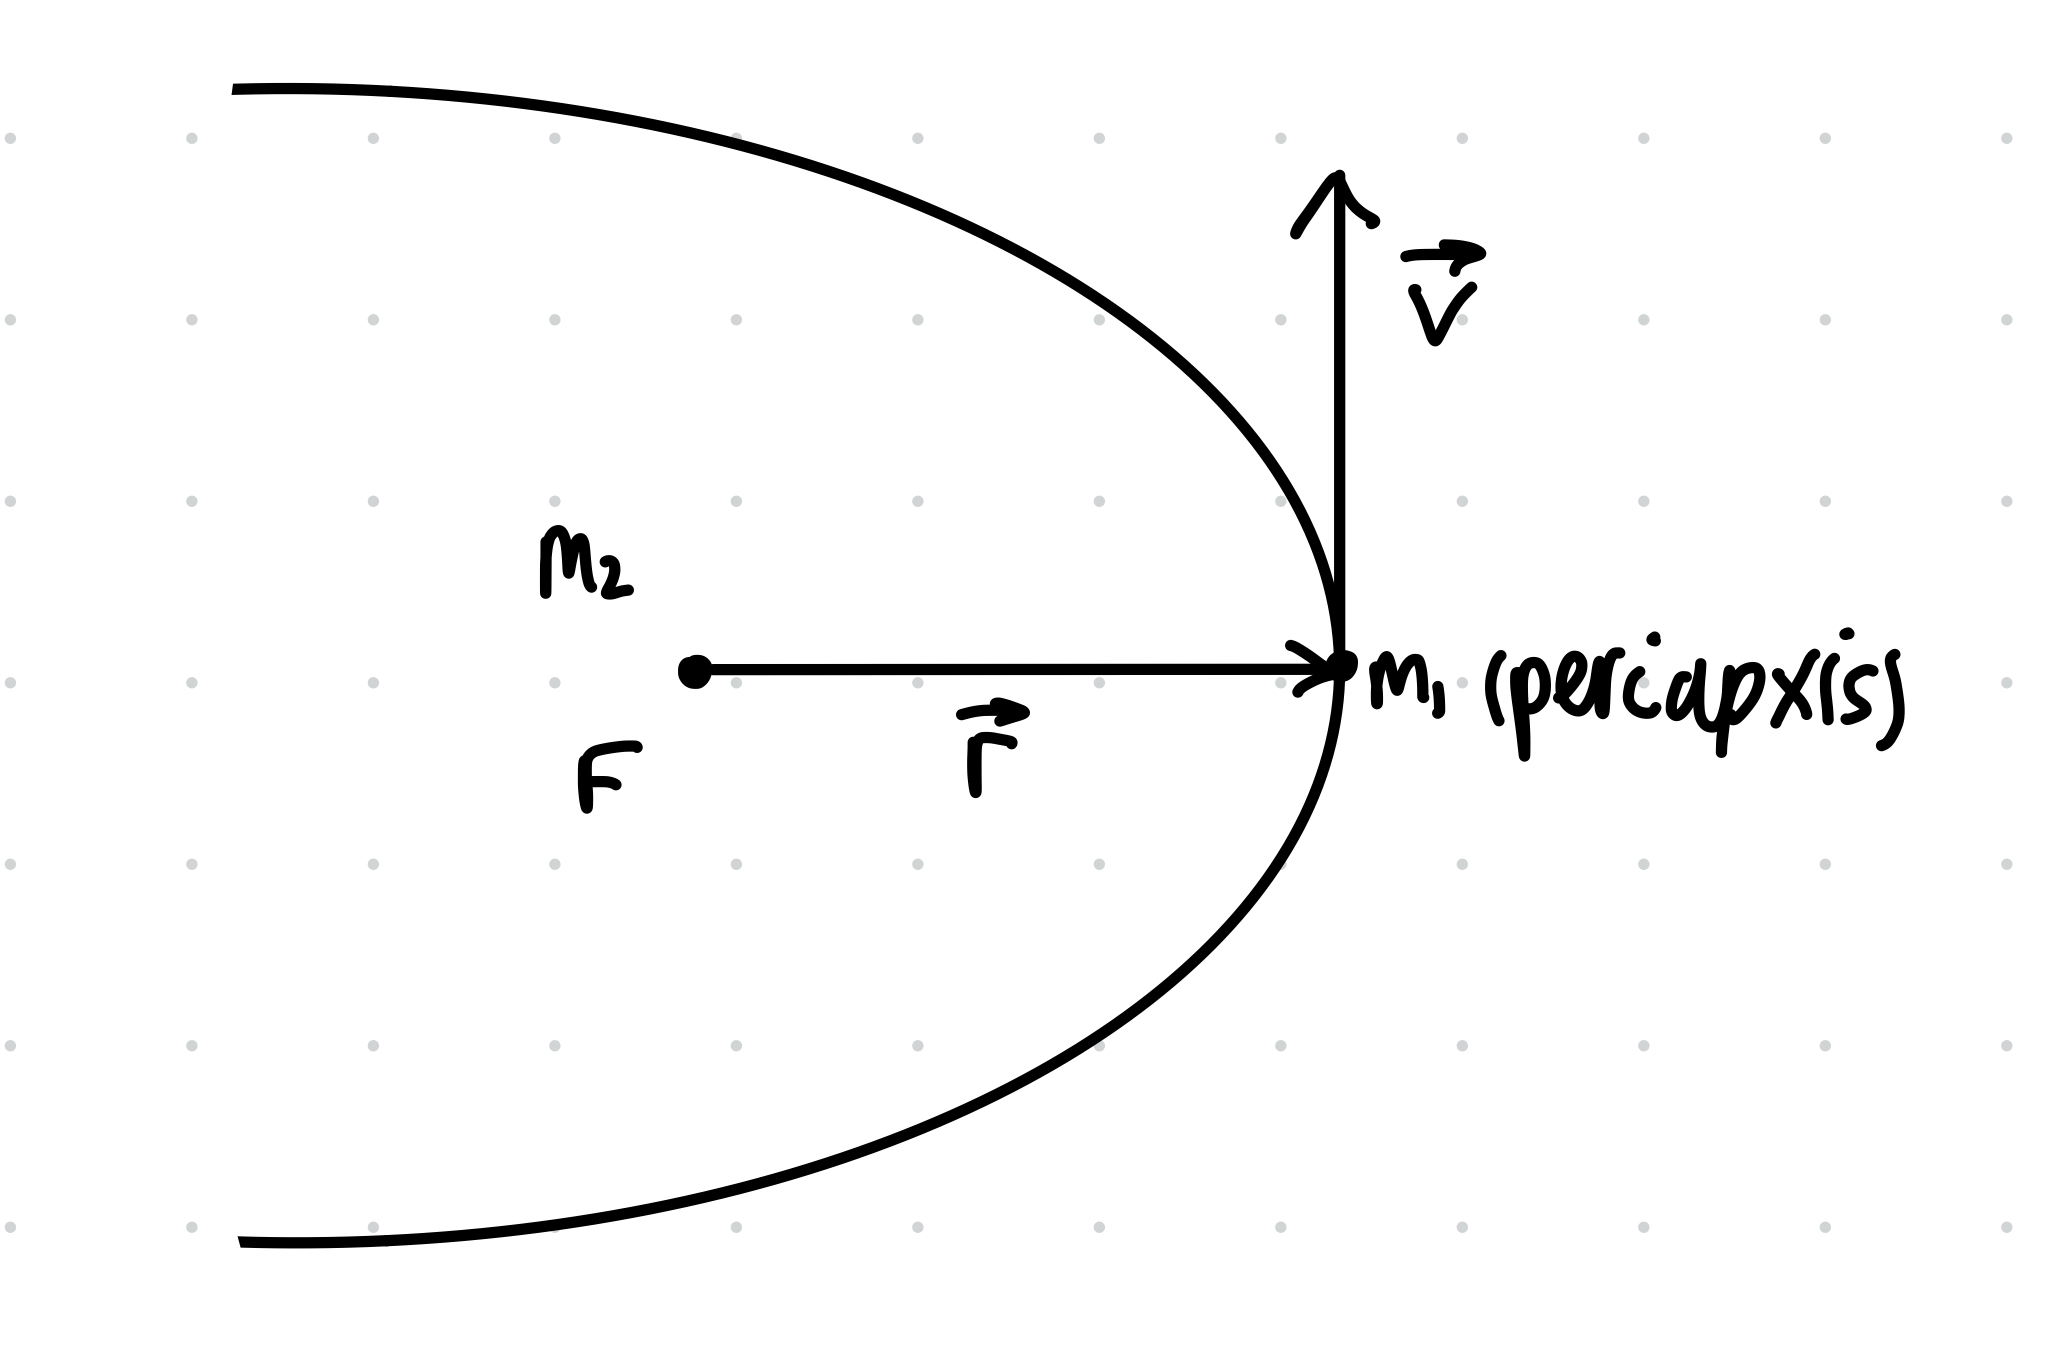
\includegraphics[width=1.0\textwidth]{Cuerpo/Imagenes/02_Ejercicio_1_2.png}
    \end{minipage}

    Tenemos que $\cn=c\hnu_3$ donde $\hnu_3=\hnu_1\wedge\hnu_2$. Supongo que $m_2\gg m_1$. Entonces:

    \begin{equation}
        \rn_c \simeq \rn_2 = 0 \tquad \rn_1 = \rn \tquad \vn = v \hnu_2
    \end{equation}
    Y por tanto $\en=\frac{1}{\mu} (\vn \wedge \cn) - \frac{\rn}{r}$. Ahora hacemos que

    \begin{equation}
        \vn \wedge \cn = \begin{vmatrix}
            \hnu_1 & \hnu_2 & \hnu_3 \\
            0 & v & 0 \\
            0 & 0 & c
        \end{vmatrix} = v c \hnu_1
    \end{equation}
    Y por tanto:

    \begin{equation}
        \en = \frac{vc}{\mu} \hnu_1 - \hnu_1 \Rightarrow \en = \ccorchetes{\frac{vc}{\mu}-1}\hnu_1
    \end{equation}
    quedando demostrado que lleva el sentido de la periapsis.
